% Final presentation -- work in progress, presented for critique.
% No animations and no screenshots of papers: equations are typeset in LaTeX.
\documentclass[aspectratio=169,11pt]{beamer}
\usepackage[utf8]{inputenc}
\usepackage[T1]{fontenc}
\usepackage[english]{babel}
\usepackage{amsmath,amssymb}
\usepackage{booktabs}
\usepackage{graphicx}
\usepackage{newunicodechar}
% Lean code is full of Unicode that typewriter fonts do not have. Each line
% maps one symbol to math mode, so Lean can be pasted into a verbatim block
% as it is (inside a [fragile] frame). Add a line for any symbol you need.
\newunicodechar{∀}{\ensuremath{\forall}}  \newunicodechar{∃}{\ensuremath{\exists}}
\newunicodechar{→}{\ensuremath{\to}}      \newunicodechar{↔}{\ensuremath{\leftrightarrow}}
\newunicodechar{∧}{\ensuremath{\land}}    \newunicodechar{∨}{\ensuremath{\lor}}
\newunicodechar{¬}{\ensuremath{\lnot}}    \newunicodechar{×}{\ensuremath{\times}}
\newunicodechar{∈}{\ensuremath{\in}}      \newunicodechar{∉}{\ensuremath{\notin}}
\newunicodechar{≤}{\ensuremath{\le}}      \newunicodechar{≥}{\ensuremath{\ge}}
\newunicodechar{≠}{\ensuremath{\ne}}      \newunicodechar{↦}{\ensuremath{\mapsto}}
\newunicodechar{ℝ}{\ensuremath{\mathbb{R}}} \newunicodechar{ℕ}{\ensuremath{\mathbb{N}}}
\newunicodechar{⟨}{\ensuremath{\langle}}  \newunicodechar{⟩}{\ensuremath{\rangle}}
\newunicodechar{λ}{\ensuremath{\lambda}}  \newunicodechar{α}{\ensuremath{\alpha}}
\newunicodechar{β}{\ensuremath{\beta}}    \newunicodechar{ε}{\ensuremath{\varepsilon}}
\usetheme{default}
\usecolortheme{seahorse}
\setbeamertemplate{navigation symbols}{}
\setbeamertemplate{footline}[frame number]
\setbeamerfont{frametitle}{size=\large}

\title{Your Title}
\subtitle{Final presentation}
\author{Your Name}
\date{October--November 2026}

\begin{document}

% The title slide carries the repository link.
\begin{frame}[plain]
  \titlepage
  \begin{center}\small
    \texttt{github.com/your-user/ai-project}
  \end{center}
\end{frame}

\begin{frame}{1 \textperiodcentered{} The question and the answer}
  \textbf{Replace.} The question, and your result in one sentence --- with its
  condition.
\end{frame}

\begin{frame}{2 \textperiodcentered{} The model}
  \textbf{Replace.} Primitives, timing, and the agent's problem.
  \[
    \max_{e \ge 0}\; a e - \frac{c}{2}\, e^{2}, \qquad a > 0,\; c > 0
  \]
\end{frame}

\begin{frame}{3 \textperiodcentered{} The result, with all its conditions}
  \textbf{Replace.} The proposition as it is stated in the paper.

  \medskip
  \textbf{Proposition 1.} If $a > 0$ and $c > 0$, the unique solution is
  $e^{*} = a/c$, and $\partial e^{*}/\partial a = 1/c > 0$.
\end{frame}

\begin{frame}{4 \textperiodcentered{} The proof: what is done and what is open}
  \textbf{Replace.} The idea of the proof, the step that was hard, and what is
  still open today. This is a progress report: say where you are.
\end{frame}

\begin{frame}{5 \textperiodcentered{} Simulations}
  \begin{columns}
    \column{.56\linewidth}
    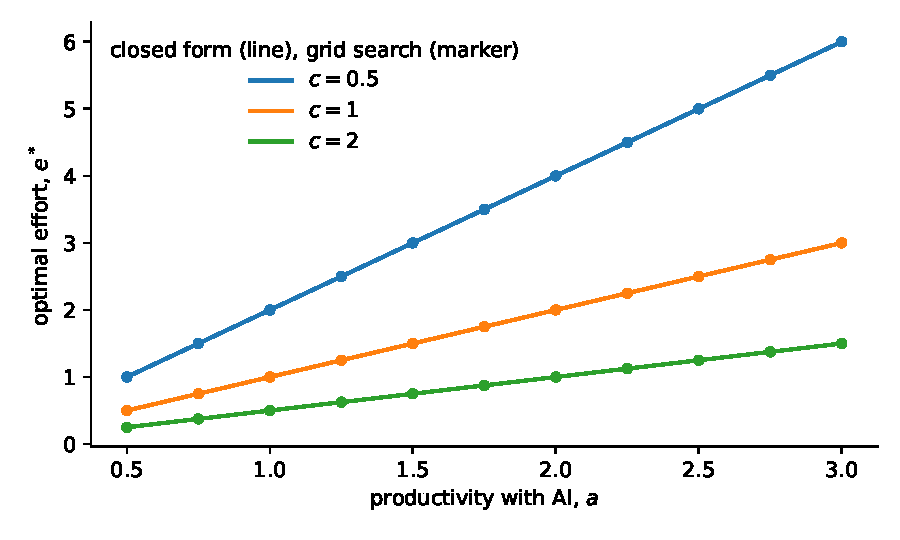
\includegraphics[width=\linewidth]{../code/figures/effort_check.pdf}
    \column{.40\linewidth}
    \textbf{Replace.} What the script checks, on which parameter range, and
    what a simulation cannot show.
  \end{columns}
\end{frame}

% Required: paper statement -> Lean statement -> what Lean verifies.
\begin{frame}[fragile]{6 \textperiodcentered{} Lean: what is verified}
  \textbf{In the paper.} $a > 0,\ c > 0 \;\Longrightarrow\; e^{*} = a/c$.

  \medskip
  \textbf{In Lean} (replace with your own statement and proof fragment):
\begin{verbatim}
theorem prop_effort (a c : ℝ) (ha : 0 < a) (hc : 0 < c) :
    a / c ∈ Set.Ici (0 : ℝ) ∧
    IsMaxOn (fun e => a * e - c / 2 * e ^ 2) (Set.Ici 0) (a / c)
\end{verbatim}
  \textbf{Replace.} How the objects and assumptions are represented, whether
  Lean verifies the paper's claim exactly or under an added hypothesis, and the
  result of the check.
\end{frame}

\begin{frame}{7 \textperiodcentered{} Where I did not believe the AI}
  \textbf{Replace.} One claim of the model, your verdict with its reason, and
  the hand derivation on screen.
\end{frame}

\begin{frame}{8 \textperiodcentered{} What I want from you}
  \textbf{Replace.} The two or three questions on which you want the class's
  critique before writing the final version.
\end{frame}

\end{document}
